\documentclass[tikz,border=6pt]{standalone}
\usepackage[T1]{fontenc}
\usepackage[utf8]{inputenc}
\usepackage{pgfplots}
\usepgfplotslibrary{groupplots}
\usetikzlibrary{calc}
\pgfplotsset{compat=1.18}
\begin{document}
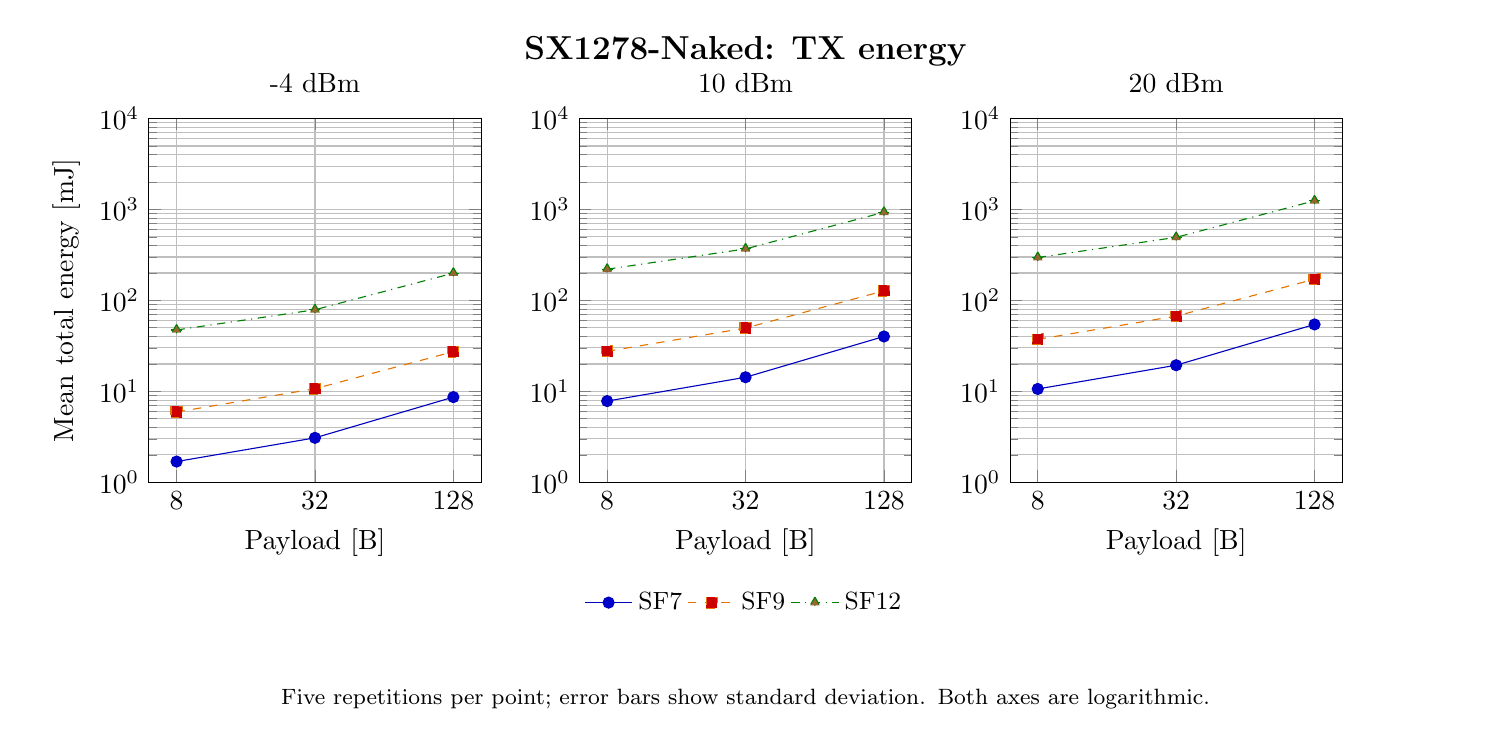
\begin{tikzpicture}
\begin{groupplot}[/pgf/number format/use comma, group style={group size=3 by 1, horizontal sep=1.25cm},
  width=5.8cm,height=6.2cm,xmode=log,log basis x=2,ymode=log,log basis y=10,ymin=1,ymax=10000,
  xtick={8,32,128},xticklabels={8,32,128},grid=both,xlabel={Payload [B]},
  legend style={draw=none,fill=none,font=\small,at={(0.5,-0.27)},anchor=north,legend columns=-1}]
% TX energy
\nextgroupplot[title={-4 dBm},ylabel={Mean total energy [mJ]}]
\addplot+[blue!75!black,solid,mark=*,error bars/.cd,y dir=both,y explicit] coordinates {(8,1.68837212) +- (0,0.00146659135) (32,3.07692699) +- (0,0.00517345996) (128,8.63406614) +- (0,0.0124506446)};
\addplot+[orange!90!black,dashed,mark=square*,error bars/.cd,y dir=both,y explicit] coordinates {(8,5.92372035) +- (0,0.00905400803) (32,10.6821764) +- (0,0.0222951026) (128,27.2821845) +- (0,0.0156306471)};
\addplot+[green!50!black,dashdotted,mark=triangle*,error bars/.cd,y dir=both,y explicit] coordinates {(8,47.280371) +- (0,0.0142417677) (32,78.9476105) +- (0,0.0812426921) (128,199.551159) +- (0,0.142354713)};
\nextgroupplot[title={10 dBm}]
\addplot+[blue!75!black,solid,mark=*,error bars/.cd,y dir=both,y explicit] coordinates {(8,7.80740176) +- (0,0.00580801825) (32,14.2768721) +- (0,0.0062922798) (128,40.1200813) +- (0,0.0273680077)};
\addlegendentry{SF7}
\addplot+[orange!90!black,dashed,mark=square*,error bars/.cd,y dir=both,y explicit] coordinates {(8,27.5244687) +- (0,0.0120890236) (32,49.6758686) +- (0,0.0166687543) (128,127.255722) +- (0,0.059481317)};
\addlegendentry{SF9}
\addplot+[green!50!black,dashdotted,mark=triangle*,error bars/.cd,y dir=both,y explicit] coordinates {(8,220.389942) +- (0,0.0392926804) (32,368.521476) +- (0,0.064906585) (128,932.131229) +- (0,0.343468272)};
\addlegendentry{SF12}
\nextgroupplot[title={20 dBm}]
\addplot+[blue!75!black,solid,mark=*,error bars/.cd,y dir=both,y explicit] coordinates {(8,10.6134235) +- (0,0.0374037732) (32,19.3631226) +- (0,0.0992117721) (128,54.396129) +- (0,0.187480486)};
\addplot+[orange!90!black,dashed,mark=square*,error bars/.cd,y dir=both,y explicit] coordinates {(8,37.2985886) +- (0,0.231234367) (32,67.2331363) +- (0,0.320304781) (128,171.178719) +- (0,0.394349978)};
\addplot+[green!50!black,dashdotted,mark=triangle*,error bars/.cd,y dir=both,y explicit] coordinates {(8,296.235648) +- (0,0.766419787) (32,493.793077) +- (0,0.269809214) (128,1247.3851) +- (0,3.1240919)};
\end{groupplot}
\node[font=\bfseries\large] at ($(group c2r1.north)+(0,0.85cm)$) {SX1278-Naked: TX energy};
\node[font=\footnotesize,align=center,text width=18cm] at ($(group c2r1.south)+(0,-2.75cm)$) {Five repetitions per point; error bars show standard deviation. Both axes are logarithmic.};
\end{tikzpicture}
\end{document}
